% Template for PLoS
% Version 1.0 January 2009
%
% To compile to pdf, run:
% latex plos.template
% bibtex plos.template
% latex plos.template
% latex plos.template
% dvipdf plos.template

\documentclass[10pt]{article}

% amsmath package, useful for mathematical formulas
\usepackage{amsmath}
% amssymb package, useful for mathematical symbols
\usepackage{amssymb}

% graphicx package, useful for including eps and pdf graphics
% include graphics with the command \includegraphics
\usepackage{graphicx}

% cite package, to clean up citations in the main text. Do not remove.
\usepackage{cite}

\usepackage{color}

% TODO temporary
\usepackage{todonotes}

% Use doublespacing - comment out for single spacing
%\usepackage{setspace}
%\doublespacing


% Text layout
\topmargin 0.0cm
\oddsidemargin 0.5cm
\evensidemargin 0.5cm
\textwidth 16cm
\textheight 21cm

% Bold the 'Figure #' in the caption and separate it with a period
% Captions will be left justified
\usepackage[labelfont=bf,labelsep=period,justification=raggedright]{caption}

% Use the PLoS provided bibtex style
\bibliographystyle{plos2009}

% Remove brackets from numbering in List of References
\makeatletter
\renewcommand{\@biblabel}[1]{\quad#1.}
\makeatother


% Leave date blank
\date{}

\pagestyle{myheadings}
%% ** EDIT HERE **


%% ** EDIT HERE **
%% PLEASE INCLUDE ALL MACROS BELOW

%% END MACROS SECTION

\begin{document}

% Title must be 150 characters or less
\begin{flushleft}
{\Large
\textbf{Object oriented implementation of Yeadon's human inertial model}
}
% Insert Author names, affiliations and corresponding author email.
\\
Christopher Dembia$^{1,\ast}$,
Jason K. Moore$^{2}$,
Mont Hubbard$^{2}$
\\
\bf{1} Mechanical Engineering, Stanford University, Palo Alto, California, USA
\\
\bf{2} Mechanical and Aerospace Engineering, University of California, Davis, California, USA
\\
$\ast$ E-mail: Corresponding cld72@cornell.edu
\end{flushleft}

% Please keep the abstract between 250 and 300 words
\section*{Abstract}
Herein we present a modern open source software implementation of a popular
mathematical method developed by M.R. Yeadon for estimating the body segment
inertia of a human body.
% Please keep the Author Summary between 150 and 200 words
% Use first person. PLoS ONE authors please skip this step.
% Author Summary not valid for PLoS ONE submissions.
%\section*{Author Summary}

\section*{Introduction}
For dynamic analyses, it is typcial to treat the human body as a collection of
linked rigid bodies. For accurate simulations and analysis the inertial
properties (mass, center of mass, and moment of inertia) of the body segments
must be estimated. Human mass, center of mass, and inertial properties have
been measured and estimated in a multitude of ways. Each method has its
advantages and disadvantages. Many methods exist including cadaver measurements
(\cite{Dempster1955}, \cite{Clauser1969}, \cite{Chandler1975}), photogrammetry,
ray scanning techniques (\cite{Zatsiorsky1983}, \cite{Zatsiorsky1990}), water
displacement (\cite{Park1999}), rotating platforms (\cite{Griffiths2005}), and
geometrical estimation of the body segments (\cite{Yeadon1990c}).
\cite{Bjornstrup1995} gives a detailed overview of mostly invasive methods up
to 1995.

Yeadon's mathematical method is quite attractive as it requires only a set of
simple measurements from a live human to give reasonable estimates of the
person's body segment parameters. Furthermore, it is based off of simple
computations and can easily be programmed to provide a quick estimates of body
segment parameters. Yeadon himself developed a Fortran program called ISEG in
his dissertation \cite{Yeadon1984a} to rapidly compute his inertia model. The
source code is available through the dissertation under the Creative Commons
Attribution-NonCommercial-NoDerivs 2.5 license but is less that adpatable for
inclusion in modern software packages for easy configuration and visualization.

We make use of Yeadon's model extensively in our dynamics research and
developed a modern object oriented program under a permissive license that
allows for easy inclusion into software packages and includes a graphical user
interface for ease of end user use.
\subsection*{Yeadon's Method}
Yeadon's mathematical model of the human body is developed by representing the
human body by a number of stadium solids and a semi ellipsoid. The ratio of the
body segment parameters are based on previous cadaver studies. He provides the
analtyical solutions for the center of mass and inertia of an individual
stadium solid. The parrlalel axis thereom is then employed to compute the
inertia properties of combinations of segments with the largest subset being
the entire body.

\subsection*{Yeadon's method}

\todo{Talk about the number of measurements and the number of joint angles}

\section*{Software design}

The input to \verb+yeadon+ consists of (1) measurements of a subject, and (2)
the joint configuration of the subject. With these two inputs, one is able to
obtain the mass properties of the subject.
The mass properties consist of the mass, center of mass, and moment of inertia
tensor. These properties can be obtained for the entire subject, or for
individual limbs of the subject. TODO any allowable configuration.

% authors may use "Analysis"
\section*{Materials and Methods}

\section*{Usage}

We demonstrate how one may use the \verb+yeadon+ package using the example of
an ice skater performing a spin. As is commonly taught in high school physics
classes when discussing the conservation of angular momentum, an ice skater
extends her arms to spin slowly, and draws them proximally to increase her
angular velocity. Since the product $I_{zz}\omega$ remains constant and $I_{zz}$
decreases, then $\omega$ must increase (with the $z$ axis directed vertically).
We can use this human inertia model to vary a model's configuration to quickly
observe the effect on $I_{zz}$. Specifically, we want to know the factor by
which an ice skater's angular velocity may increase when she draws her arms in
from a directly outward position.

We begin by describing how \verb+yeadon+ is obtained and installed, then
discuss the two ways that \verb+yeadon+ can be used to approach this problem.

\subsection*{Obtaining and installing the software}

The package, along with its documentation, is distributed through the Python
Package Index. Accordingly, the package can be downloaded and installed easily
from the command line on a user's machine using the \verb+pip+ package:

\begin{verbatim}
$ pip install yeadon
\end{verbatim}

There are two ways to use the package: through methods of the \verb+Human+
class, or through an interactive command-line user interface. We cover both.



\subsection*{The Human class}

\begin{verbatim}
import yeadon as y
h = y.Human('female1.txt')
\end{verbatim}

This constructs the \verb+Human+ with the segment dimensions as given in the
\verb+female1.txt+ input file. This human has the default configuration, in
which all joint angles are zero. This human can be visualized by executing the
following:

\begin{verbatim}
h.draw()
\end{verbatim}
\todo{is draw() correct}

Figure \ref{fig:femaledefault} shows this Human

TODO show the use of some other methods, for instance averaging and scaling.

\subsection*{The command-line user interface}


-dev for python2.7
-assume unix machine
-dist through pip
-how to install
-two ways to use.


\todo{Measurement figure}

% Do NOT remove this, even if you are not including acknowledgments
\section*{Acknowledgments}
TODO nsf disclaimer
%\section*{References}
% The bibtex filename
\bibliography{humaninertia}

\section*{Figure Legends}
%\begin{figure}[!ht]
%\begin{center}
%%\includegraphics[width=4in]{figure_name.2.eps}
%\end{center}
%\caption{
%{\bf Bold the first sentence.}  Rest of figure 2  caption.  Caption 
%should be left justified, as specified by the options to the caption 
%package.
%}
%\label{Figure_label}
%\end{figure}

\begin{figure}[!ht]
\begin{center}
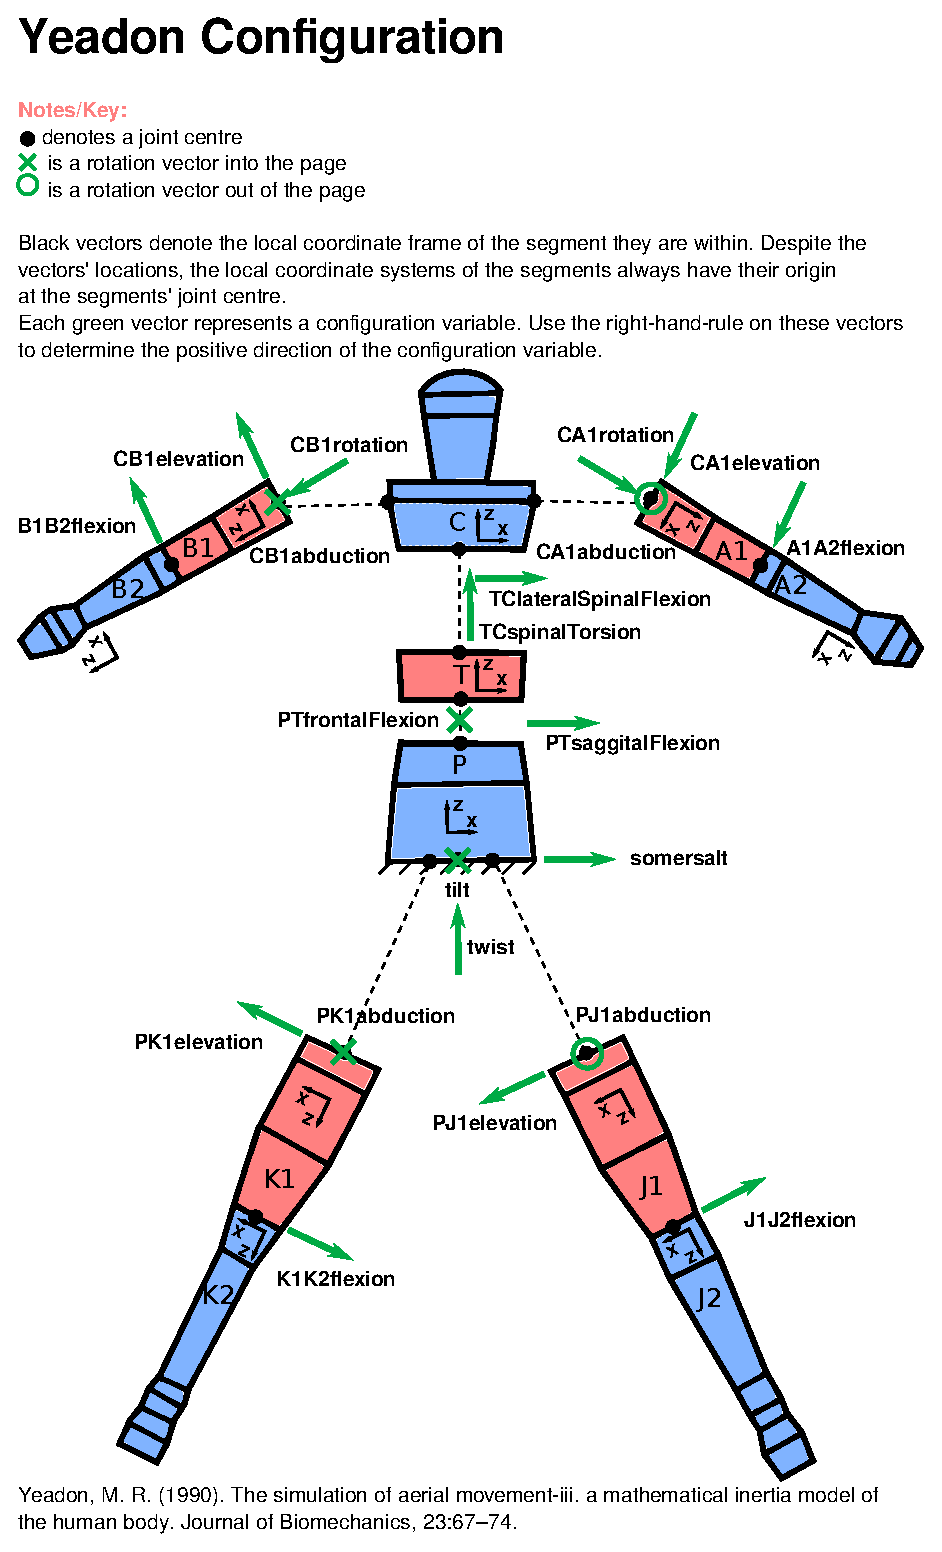
\includegraphics[width=4in]{configuration.eps}
\end{center}
\caption{
{\bf Bold the first sentence.}  Rest of figure 2  caption.  Caption 
should be left justified, as specified by the options to the caption 
package.
}
\label{fig:config}
\end{figure}

\begin{figure}[!ht]
\begin{center}
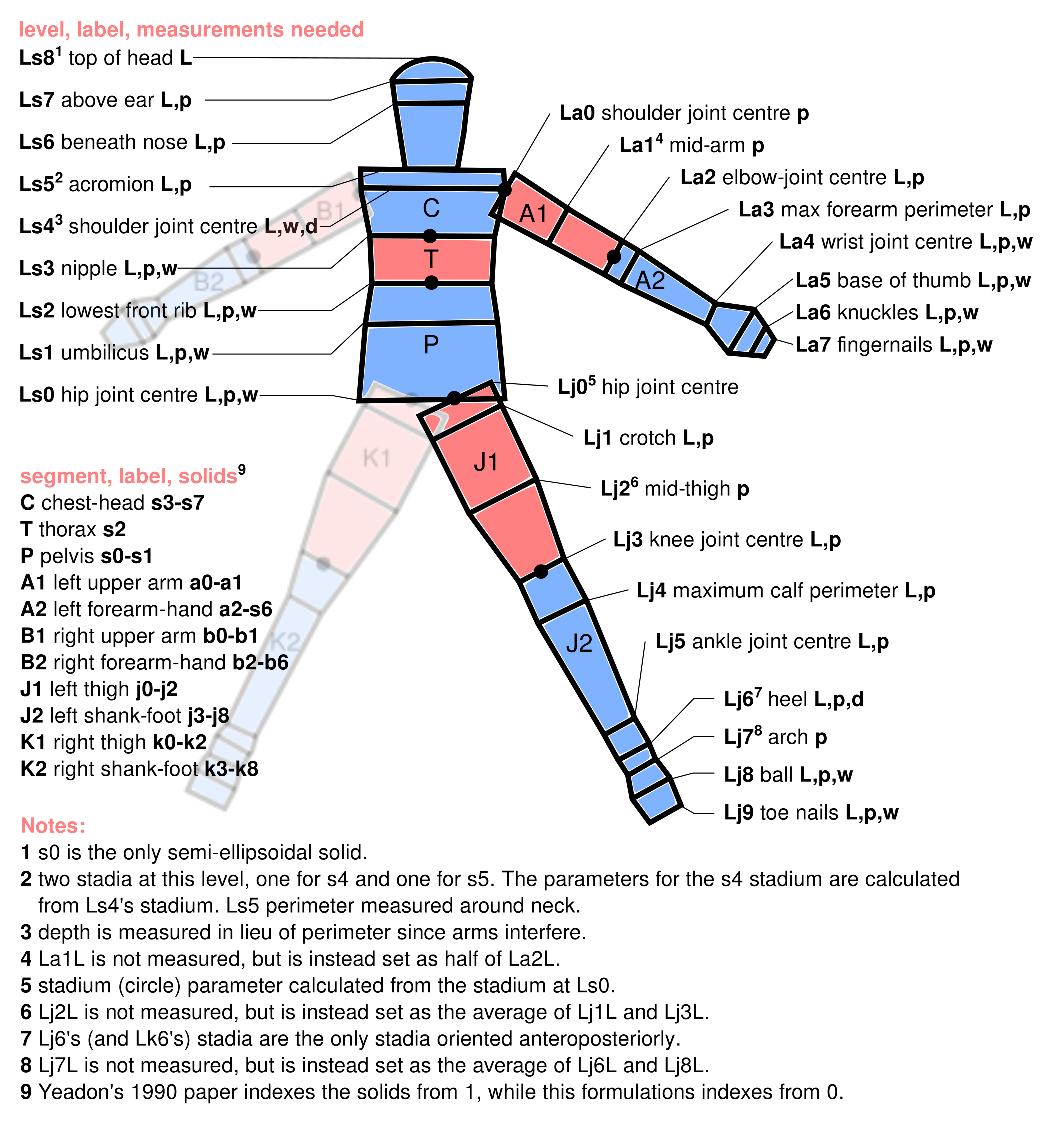
\includegraphics[width=4in]{measurements.eps}
\end{center}
\caption{
{\bf Bold the first sentence.}  Rest of figure 2  caption.  Caption 
should be left justified, as specified by the options to the caption 
package.
}
\label{fig:meas}
\end{figure}

\begin{figure}[!ht]
\begin{center}
    \missingfigure{femaledefault}
%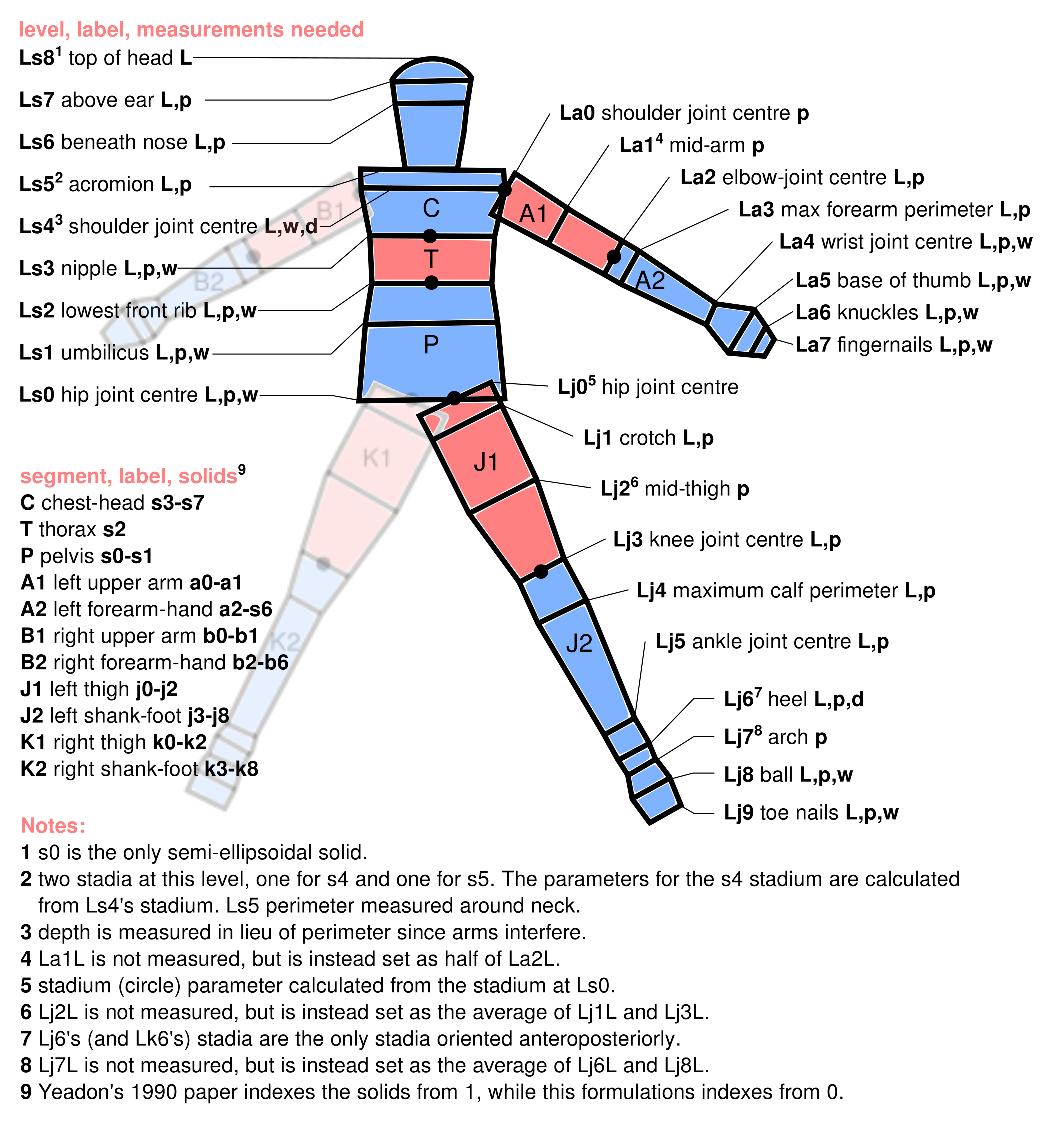
\includegraphics[width=4in]{measurements.eps}
\end{center}
\caption{
{\bf Bold the first sentence.}  Rest of figure 2  caption.  Caption 
should be left justified, as specified by the options to the caption 
package.
}
\label{fig:femaledefault}
\end{figure}

\section*{Tables}
%\begin{table}[!ht]
%\caption{
%\bf{Table title}}
%\begin{tabular}{|c|c|c|}
%table information
%\end{tabular}
%\begin{flushleft}Table caption
%\end{flushleft}
%\label{tab:label}
% \end{table}

\end{document}
